% !TeX root = ../main.tex
% Add the above to each chapter to make compiling the PDF easier in some editors.

\chapter{Introduction}\label{chapter:introduction}

This chapter includes an explanation of the exact problem we are addressing, and why, a brief overview of our solution, and the attacks we are trying to fend off.

% nicht wissenschaftliche Teil, zero trust ist jetzt ein Ding, immer mehr embedded ohne TPM (z.B. Gartner Studien)

\section{Motivation}

% Which area this thesis is talking about (Zero Trust)

Modern trust relationships, such as Zero Trust~\cite{isaca2021}, require trustworthy platforms, which can reliably report their system state.
In such models, trust is no longer implicitly assumed, e.g., by the fact that a device is located within the boundaries of a company.
Instead, each device is considered compromised until proven otherwise on a per-request basis for resource (e.g., printers) and data access~\cite{Rose2020}.

% Primer on remote attestation

This is solved by remote attestation.
In the simplest case, there is a prover and a verifier, as depicted in \autoref{fig:ra_simple}.
The challenge is that the verifier observes nothing but bytes from the prover, and while a benign prover will tell the truth about its state, a compromised prover will lie about its state and claim a trustworthy one.
Therefore, the verifier must establish trust to a helper component on the prover's side.
This component must be manufacturer-controlled so that it cannot be modified without the involvement of the manufacturer, who identifies themselves to a verifier by signing and storing a certificate on the helper components supplied by them.
Consequently, the component attests the state of the prover's machine, from which the verifier can deduce whether the prover can be considered trustworthy.

\begin{figure}[htpb]
  \centering
  \includegraphics[width=0.5\linewidth]{figures/remote_attestation_process.pdf}
  \caption{Simplified remote attestation process.}\label{fig:ra_simple}
\end{figure}


% TPMs become more important

For example, this can be done with a \acf{TPM} on the prover's side. They rise in their deployments and importance, e.g., in 2013 the President's Council of Advisors on Science and Technology encourages the adoption of TPMs~\cite{usa}, and Microsoft publicized that they require a TPM module for Windows~11 in 2021~\cite{win11req}.
They provide remote attestation mechanisms of system states, and their applications are still expanding beyond their traditional use-cases. For example, they are used in anti-cheat software for games~\cite{valorant}.

% Short intro why fTPMs were introduced (for weak devices, exactly our target platform)

A \acf{dTPM} increases cost and hardware complexity---especially for embedded platforms.
\Acfp{fTPM} running in a \acp{TEE} can be used to provide similar security guarantees as a \ac{dTPM} chip.

% Why establishing trust in an fTPM is harder than in a dTPM

For a \ac{dTPM}, which consists of an independent hardware unit manufactured by a single manufacturer and is directly activated by power, it is sufficient to identify its manufacturer and understand their provided guarantees.
In contrast, an \ac{fTPM} runs atop other firmware components and is started later in the boot chain, making its security dependent on the underlying firmware stack.
Consequently, trust in an \ac{fTPM} depends on trusting the entire stack beneath it due to the possibility that its underlying firmware might alter or compromise the \ac{fTPM}.

% What's the difficulty of establishing trust to an fTPM?

However, while a TPM-compliant component provides an infrastructure with which trust in it can be established remotely, i.e., an endorsement (key) certificate~(EKcert), the underlying firmware stack is not represented by this.

% How it currently works for fTPMs

Currently, this is solved by the manufacturer providing not only the fTPM, but also the entire underlying firmware stack.
Consequently, by establishing trust to the manufacturer of the fTPM, one can implicitly trust the underlying firmware as well by assuming they also originate from this manufacturer.
This is possible since in the most general sense, one can derive from an endorsement certificate the endorser, i.e., manufacturer, and if the attester trusts the manufacturer and the guarantees he provides, trust is established to his provided components.

\begin{figure}[htpb]
  \centering
  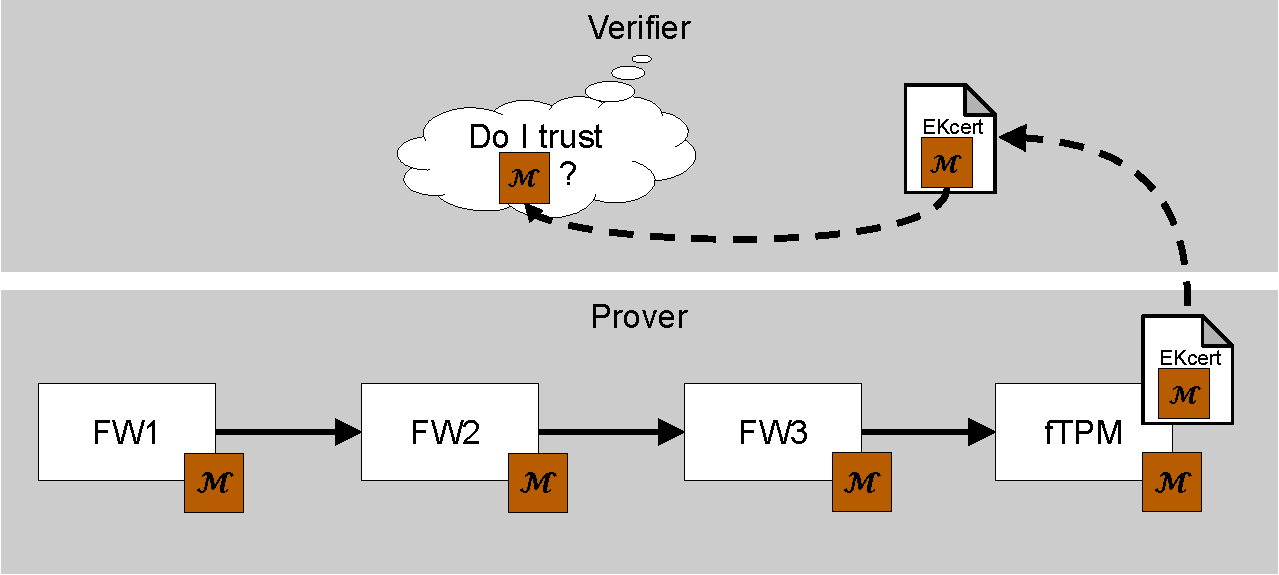
\includegraphics[width=1\linewidth]{figures/current_state.pdf}
  \caption{The naive process how a verifier establishes trust to an \ac{fTPM}, which is in fact done by trusting its manufacturer. The brown markers indicate a manufacturer. The firmware~(FW) and the fTPM were built by manufacturer \(\mathcal{M}\), and the EK certificate indicates this manufacturer.}\label{fig:current_state}
\end{figure}


This process is illustrated in figure \autoref{fig:current_state}.
The prover's box shows its boot chain, the verifier's box shows how it evaluates the trustworthiness against the prover's boot chain.
The verifier trusts the entire firmware chain if he trusts the manufacturer of each individual component.
Note how the verifier must assume that the manufacturer of the firmware components is the same as the manufacturer of the fTPM\@.
To the best of our knowledge, this is what manufacturers like Intel and AMD implement for their \acp{fTPM}, as confidence in their \acp{fTPM} is also only established through an EKcert.

% Summary with limitations

In summary, with the current approach, the endorser, usually a CPU manufacturer, provides the firmware up to the fTPM and guarantees the firmware is not modifiable by untrusted parties.
This enables trust to the other firmware components this manufacturer provided without knowing the firmware.
This approach is limited, as with this mechanism, independent verifiers have to blindly trust the firmware manufacturer, which drastically limits trust relationships.

\section{Goal}

We establish an independently verifiable fTPM stack, rooted in a hardware root of trust, that can be leveraged in a zero trust environment with little hardware requirements and no compromising on security.
The goal of this approach is to break the requirement of the underlying firmware and the fTPM to originate from the same manufacturer, by providing the exact firmware component identities to the verifier, such that it can decide for itself whether they are trustworthy without relying on their manufacturer.
Instead, it is sufficient to trust the independent manufacturer of the hardware root of trust, which in contrast requires no assumptions.

% Short introduction to DICE

One mechanism enabling firmware attestation is the \ac{DICE}, focusing on resource-constrained devices.
Although this mechanism shifts trust from the firmware provider to the hardware provider by allowing firmware attestation through a hardware root of trust, the exclusive use of this integrated solution is unsuitable for large dynamic systems, for example Linux based devices.
Nevertheless, the advantage is that the identity of each component of the firmware boot chain is represented.

% How we try to overcome these limitations

We propose a hybrid solution, combining the advantages of \ac{DICE} and \acp{fTPM}, yielding an independently verifiable certificate chain representing the boot chain up to and including the \ac{fTPM}.
This enables a verifier to establish trust in an \ac{fTPM} if the underlying firmware is benign as well and thus, providing a way to independently assess the properties of the \ac{fTPM}.
% The conceptual basis for this is to attest the software stack of the TPM itself, and thus providing a way to independently assess the properties of the fTPM.

%Current \ac{fTPM} implementations require additional security measures to not leak state between reboots and different software versions.
%The final concept should provide a comprehensive guideline to implement an fTPM, which accounts for such an environment and reflect any relevant information through remote attestation.

The research questions we aim to answer are listed below.
\begin{itemize}
  \item What constitutes the identity of an fTPM\@? %(e.g., hash, configuration, boot chain)
  \item How to combine the DICE and TPM infrastructure? %(e.g., AliasCert $\cup$ EKcert)
  \item How to manage an fTPM's persistent data securely? %(e.g., flush data on update)
  \item How to enable privacy for this attestation mechanism?
\end{itemize}

% Prover and verifier can take both roles for mutual attestation

% Chaining the underlying firmware identities with the endorsement identity

\section{Threat Model}

% https://trustedfirmware-a.readthedocs.io/en/latest/threat_model/threat_model.html

% Attacker model: What an attacker can do (abilities) and cannot do (limits)

The attacker we are interested in is able to replace the fTPM or one of its predecessor components.
Therefore, there is a risk that a remote party trusts a firmware TPM that is in fact not trustworthy.
For example, an attacker could install a malicious update of a relevant firmware component on the target device.
However, we assume that the attacker is only able to do this before or during the boot process of the device, but not afterwards.
Hardware attacks, side-channel attacks, control-flow attacks, and denial-of-service attacks are out-of-scope.

For the network, we assume the Dolev-Yao attacker model~\cite{Dolev1983}.
That is, we consider an attacker who has the ability to perform any active or passive attack on the network.
The attacker may also have control over parts or the entire network, e.g., all routers, switches, and connections.
Last, they cannot break cryptographic primitives, e.g., encryption, signing, and hashing.

\section{Security goals}

In this section, we want to formally describe the security goals of our solution so that we can later briefly discuss whether and how we achieve the corresponding objectives.

\begin{itemize}
  \item{\textbf{Compromised fTPM cannot fake its identity}\\
  A compromised fTPM must not be able to lie to the verifier about its identity.
  It is sufficient for a lie to be recognized, and the verifier can consequently classify the verifier's fTPM as untrustworthy.}
  % Does not have access to OP-TEE's private key, code in user mode does not have access to data in kernel mode

  \item{\textbf{Small root of trust}\\
  A root of trust of small size, e.g., in the means of code size, hardware size, and complexity, yields a small attack surface~\cite{Singaravelu2006}.
  This is due to the fact that a small component yields less potential implementation errors, and its approaches to guarantee specific security properties are more manageable.}
  % DICE, its design, not concrete HW, its protection of the \ac{UDS}
  
  \item{\textbf{Isolation of fTPM storage}\\
  Data must only be accessible or modifiable within the boundaries of the TPM access controls, i.e., the TPM commands defined by its specification~\cite{tpm20}.}
  This includes the protection against other trusted applications running in the same TEE\@.
  
  \item{\textbf{Protect fTPM data against downgrade attacks on the fTPM}\\
  The current storage of the fTPM should be sealed to the identity of the fTPM's identity, such that when the fTPM is modified, e.g., by a downgrade attack, even the fTPM cannot access its old data anymore.}

  \item{\textbf{Privacy of remote attestation process}\\
  The verifier should be able to establish trust to an fTPM without having to know the identity of the fTPM, i.e., its EK\@.}
\end{itemize}

\section{Environment}

This work was created at the `Fraunhofer-Institut für Angewandte und Integrierte Sicherheit AISEC' in Garching.
It is part of the `Fraunhofer Society for the Promotion of Applied Research e.~V.', which is an organization distributed over Europe with main focus on applied research.
In the roughly 35 years of its existence, it rose to become the largest research institute in Europe with around 30,000 employees.

\section{Outline}

In the \nameref{chapter:background}, we provide knowledge necessary for a better understanding of the subsequent parts of this thesis.
Afterwards, we discuss \nameref{chapter:related_work}, i.e., attacks on TPMs to further motivate this work, approaches to hardening TPMs, and work that enables remote attestation similar to ours.
Under \nameref{chapter:methodology}, we explain the concept of our solution and subsequently present our proof-of-concept \hyperref[chapter:implementation]{implementation}.
Finally, we \hyperref[chapter:discussion]{discuss} our design and implementation, rounded off by \nameref{chapter:future_work_and_conclusion}.
